\chapter[Análise dos Resultados]{Análise dos Resultados}
\label{chap:Análise dos Resultados}
Neste capítulo são apresentados os resultados obtidos através dos testes de usabilidade e experiência de usuário realizados no aplicativo Multilind. Os testes seguiram a estrutura de uma pesquisa-ação, que envolve a concepção e a realização de uma 
investigação em associação com a ação ou resolução de um problema conhecido, como descrito no \hyperref[sec:Metodologia de Analise de Resultados]{Capítulo 4}. No decorrer da análise de resultados, destacam-se as \hyperref[sec:Personas]{Personas} 
(Seção \hyperref[sec:Personas]{6.1}) envolvidas, os \hyperref[sec:Cenários de Uso]{Cenários de Uso} (Seção \hyperref[sec:Cenários de Uso]{6.2}) e \hyperref[sec:Práticas Adotadas]{Práticas Adotadas} (Seção \hyperref[sec:Práticas Adotadas]{6.3}) 
durante o protocolo de pesquisa-ação. Por fim, são apresentadas as considerações finais acerca dos resultados obtidos.

\section{Personas}
\label{sec:Personas}
Como descrito no Capítulo \hyperref[sec:Persona]{2}, as personas são representações semifictícias que detêm perfis desejáveis para os testes nos aplicativos. Esses perfis são definidos por características específicas que orientam a seleção da amostra, 
garantindo a consistência dos resultados. 

Com o intuito de avaliar a usabilidade e a experiência do usuário no aplicativo Multilind, foram realizadas provas de conceito para ambas as versões do aplicativo: a última versão (v1.4.0) e a versão com melhorias propostas. Para esse propósito, 
foram selecionados cinco usuários que representam diferentes perfis de personas, permitindo uma avaliação abrangente.

A escolha de cinco usuários orienta-se por uma abordagem amplamente adotada. \citeonline{usabilitytest} argumenta que realizar testes com cinco usuários é suficiente para identificar a maioria dos problemas de 
usabilidade. Ele baseia essa conclusão em estudos empíricos e observações, sugerindo que a descoberta de problemas de usabilidade tende a estagnar após o quinto participante, com poucos benefícios 
extras sendo obtidos com participantes adicionais.

O primeiro ciclo de testes foi realizado com objetivo de coletar métricas e informações de usabilidade e experiência do usuário no aplicativo Multilind implantado. Já o segundo ciclo de testes visou validar as 
melhorias propostas, no intuito de obter insumos, via análise dos resultados obtidos, sobre a pertinência dessas melhorias, na visão do público alvo. Dependendo do grau de concordância dos usuários, se alto, a 
melhoria é vista como pertinente, sendo mantida no plano de ação de melhorias a serem implementadas efetivamente no aplicativo. Em caso de baixa concordância, vistas como não pertinentes. Portanto, removidas 
do plano de ação de melhorias. Em caso de concordância parcial (ou seja, de grau intermediário), há adequação das melhorias considerando os apontamentos conferidos. 

Todos os participantes participaram voluntariamente, de acordo com os termos estabelecidos no  TERMO DE CONSENTIMENTO LIVRE E ESCLARECIDO (TCLE), que foi adaptado do modelo da Universidade de Araraquara \cite{tcle}, 
disponível no Apêndice \ref{ApendiceB} para consulta.

\section{Cenários de Uso}
\label{sec:Cenários de Uso}
Durante os ciclos de testes de usabilidade, foram avaliadas sete funcionalidades principais do aplicativo Multilind. Essas funcionalidades foram escolhidas com o objetivo de identificar os aspectos-chave do 
aplicativo. Os participantes foram solicitados a interagir com cada uma dessas funcionalidades e fornecer feedback instantâneo sobre suas percepções. As funcionalidades testadas incluem:

\begin{itemize}

	\item Visualizar línguas através do mapa (F01): Os usuários podem visualizar as diferentes línguas representadas geograficamente no mapa do aplicativo.

    \item Ver detalhes de uma língua ao clicar em um ponto no mapa (F02): Ao clicar em um ponto específico no mapa, os usuários podem acessar informações detalhadas sobre uma língua específica.
    
    \item Visualizar línguas por ordem alfabética (F03): Esta funcionalidade permite aos usuários visualizar uma lista de línguas ordenadas alfabeticamente.
    
    \item Visualizar línguas por família linguística (F04): Os usuários podem explorar as línguas agrupadas por famílias linguísticas.
    
    \item Ver dicionário de palavras de uma língua específica (F05): Esta funcionalidade permite aos usuários acessar o dicionário de palavras de uma língua específica.
    
    \item Ver tradução de uma palavra para o português formal (F06): Os usuários podem traduzir uma palavra de uma língua indígena para o português formal.
    
    \item  Visualizar imagens relativas às palavras de uma língua (F07): Esta funcionalidade permite aos usuários visualizar imagens relacionadas às palavras de uma língua específica.

\end{itemize}

\section{Práticas Adotadas}
\label{sec:Práticas Adotadas}
Durante a execução dos testes de usabilidade, foi utilizado o Maze, apresentado na seção \hyperref[{sec:Maze}]{3.2.4.1}, que permite a realização de testes remotos. Essa ferramenta possibilita a gravação da tela do computador ou celular 
durante o teste. Os participantes foram orientados a realizar as tarefas descritas na Seção \hyperref[sec:Cenários de Uso]{6.2} nos protótipos do aplicativo.

Após cada teste, a plataforma Maze gera um relatório completo, contendo métricas detalhadas coletadas durante a sessão e uma síntese dos resultados gerais. Esse resumo pode ser visualizado na Figura \ref{fig31}, que apresenta a duração das interações, a taxa de sucesso e 
a incidência de cliques incorretos em diferentes fluxos de funcionalidades.

\begin{figure}[h!]
	\centering
	\caption{Resumo dos resultados na plataforma Maze}
	\begin{adjustbox}{center}
		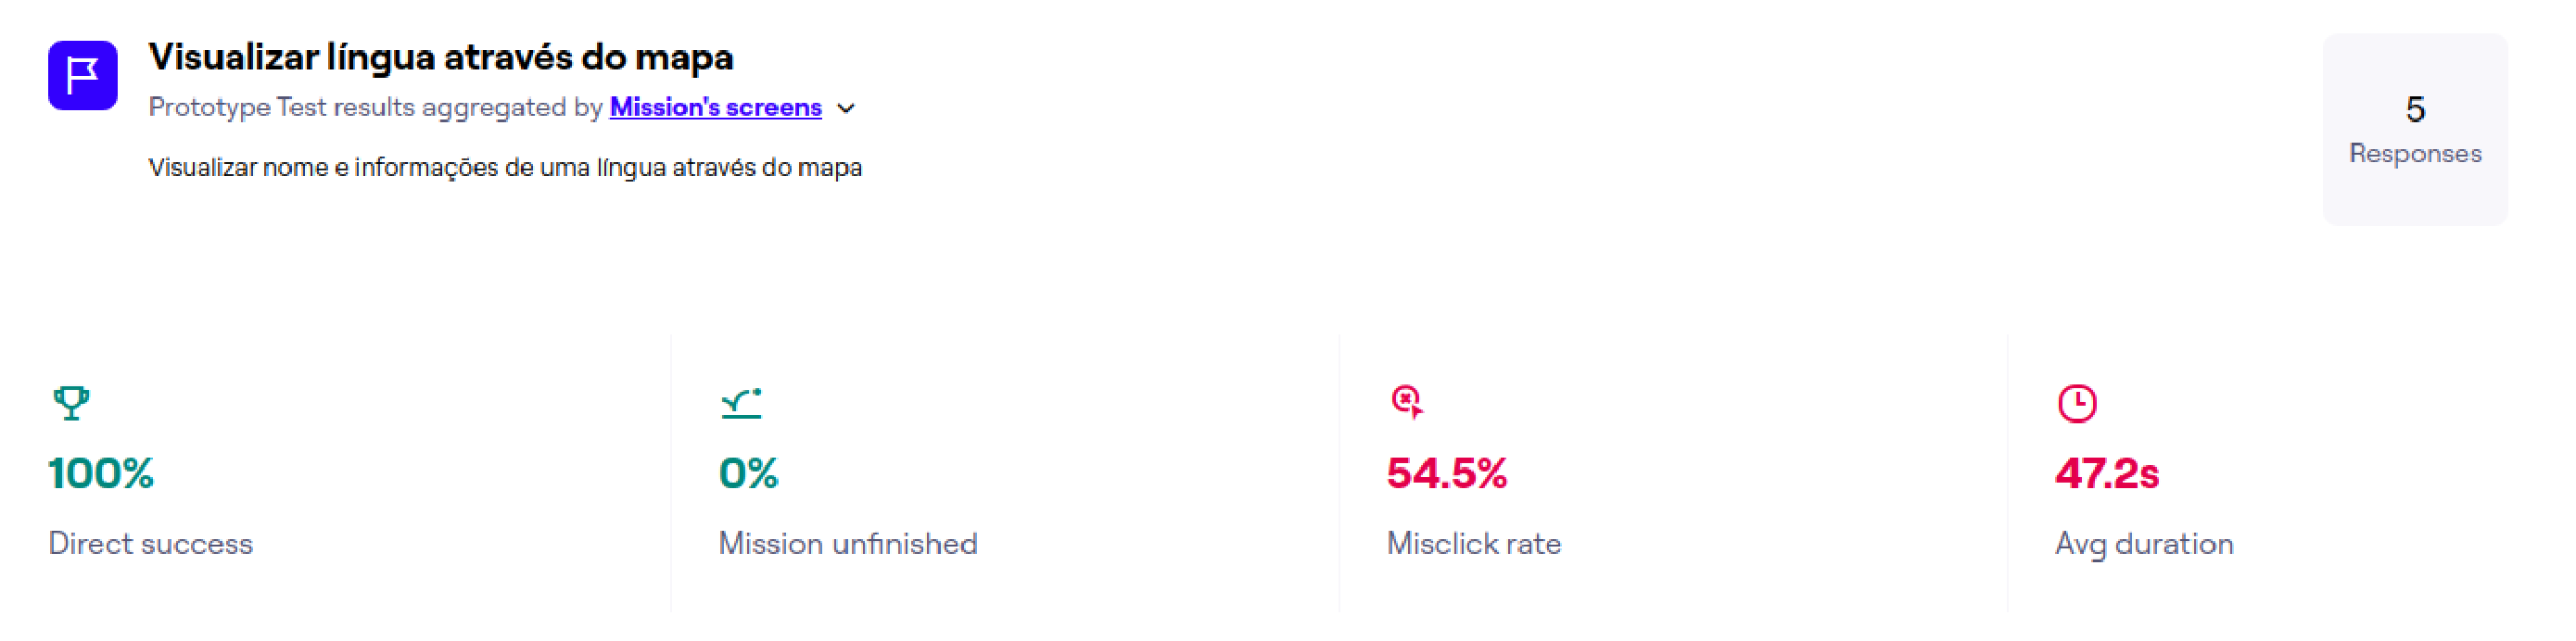
\includegraphics[width=1\textwidth]{figuras/maze.eps}
	\end{adjustbox}
	\begin{tablenotes}[flushleft]
		\centering
		\item \textit{Fonte:} Autora.
	\end{tablenotes}
	\label{fig31}
\end{figure}

A Figura \ref{fig32} fornece informações de sessão específicas por participante, incluindo o tempo gasto durante a execução das tarefas e o resultado obtido, indicando se foi um sucesso direto ou indireto.

O sucesso direto é caracterizado pela capacidade do participante de concluir a tarefa seguindo o caminho esperado, ou seja, o fluxo de telas definido para que o participante complete uma tarefa específica. Por outro lado, o sucesso indireto ocorre quando o usuário completa a tarefa 
sem seguir esse caminho previamente definido, seja passando por um fluxo diferente ou percorrendo um número maior de telas antes de concluir.

\begin{figure}[h!]
	\centering
	\caption{Resultados por participante na plataforma Maze}
	\begin{adjustbox}{center}
		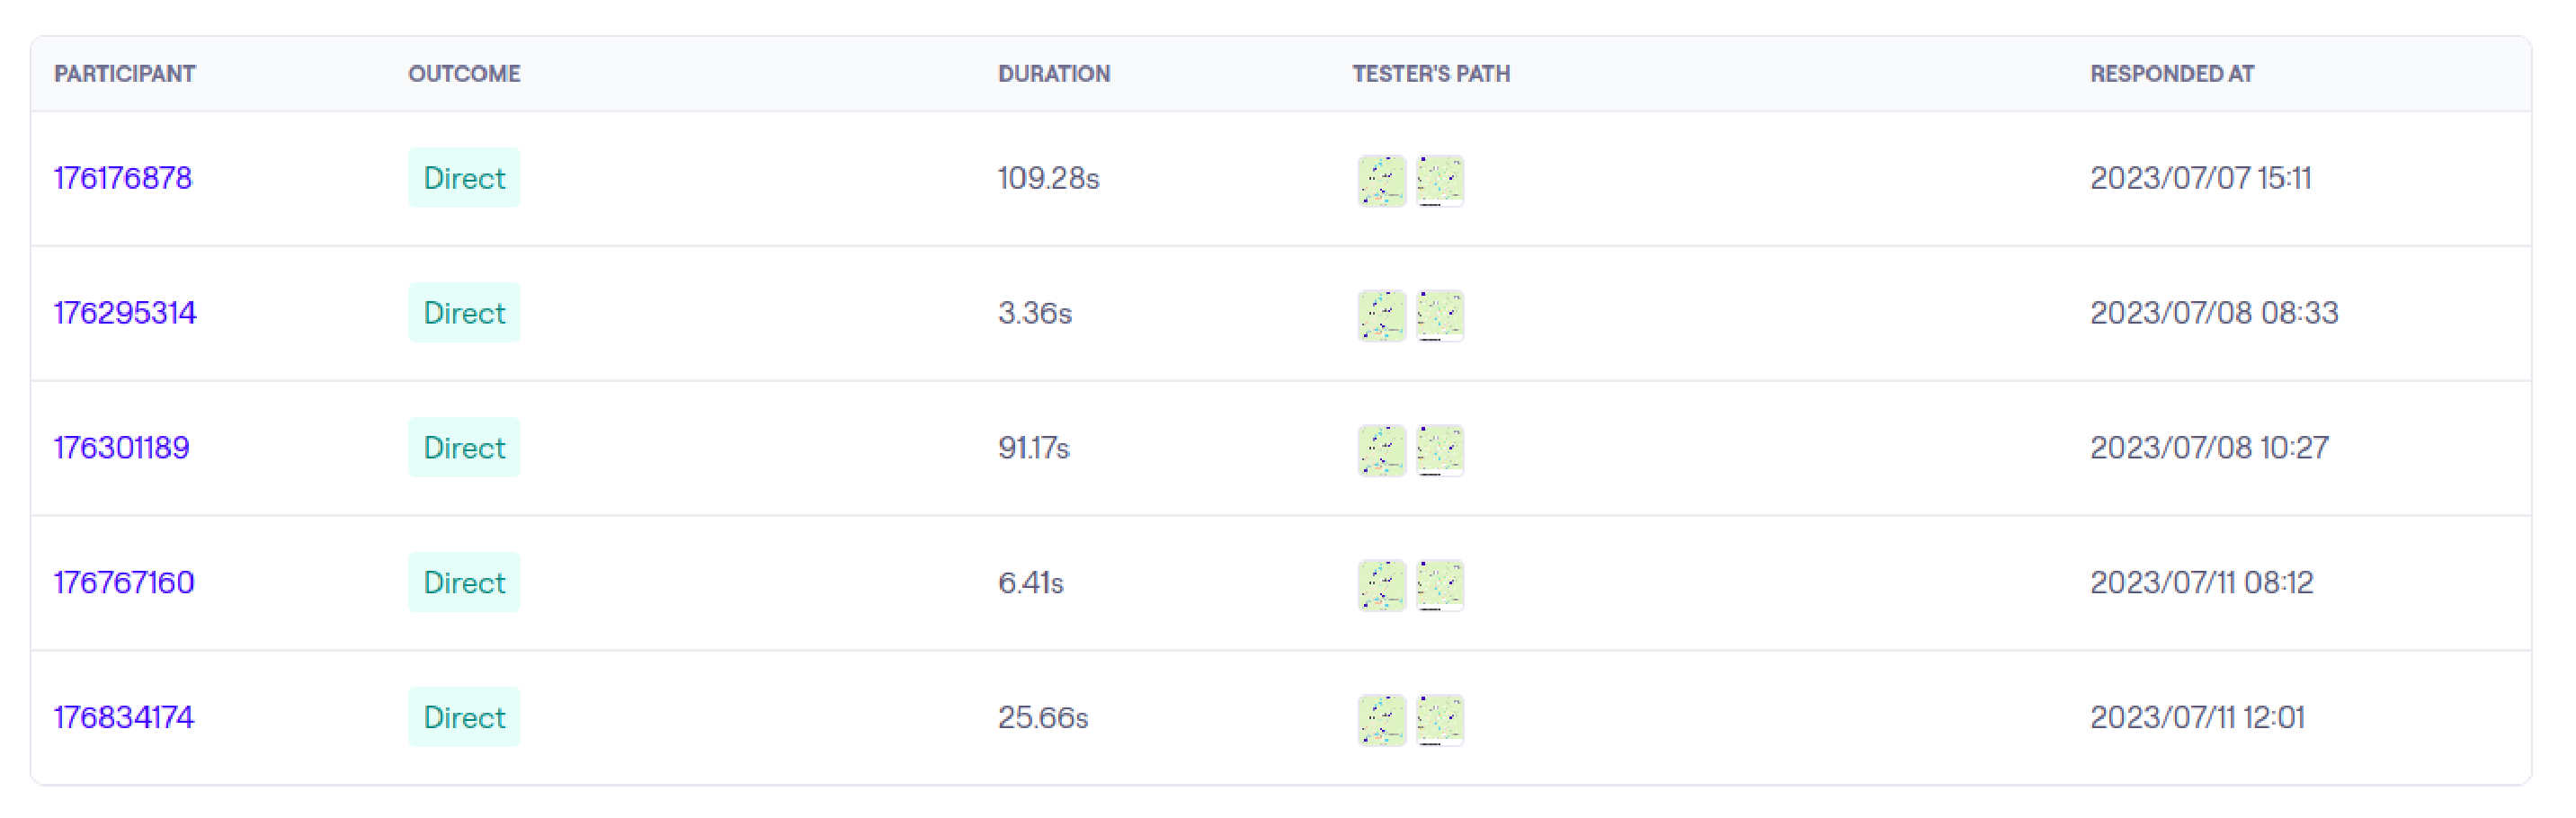
\includegraphics[width=1\textwidth]{figuras/maze2.eps}
	\end{adjustbox}
	\begin{tablenotes}[flushleft]
		\centering
		\item \textit{Fonte:} Autora.
	\end{tablenotes}
	\label{fig32}
\end{figure}

Além disso, ao final dos testes, foi aplicado um questionário baseado no Questionário \textit{Attrakdiff} para avaliar a experiência do usuário no aplicativo Multilind. Este questionário foi detalhadamente explicado na seção \hyperref[sec:Medicao2]{2.3.1}.

\section{Primeiro Ciclo de Testes}
\label{sec:Primeiro Ciclo}
O primeiro ciclo de testes foi conduzido com cinco usuários, com o objetivo de avaliar as funcionalidades na versão v1.4.0 do aplicativo. Durante esse ciclo, os participantes realizaram as tarefas enquanto forneciam \textit{feedback} instantâneo sobre suas experiências durante o uso 
do aplicativo. Os principais pontos levantados foram:

\begin{itemize}
	\item Falta de orientação no primeiro uso: foi observado pelos participantes a falta de instruções claras e orientações sobre como navegar e utilizar as funcionalidades no primeiro acesso ao aplicativo;
	\item Maior clareza na opção de visualizar línguas por família linguística: alguns participantes relataram dificuldades em localizar a opção para visualizar as línguas agrupadas por família linguística;
	\item Ausência de cores: usuários relataram sentir que a aplicação carecia de uma paleta de cores mais vibrantes para torná-la visualmente atraente, e
	\item Carência de informações a respeito de como contribuir: houve interesse manifestado por alguns participantes em contribuir com a base de dados do aplicativo. Entretanto, sentiram falta de informações a respeito 
	de como contribuir no aplicativo.
\end{itemize}

\subsection{Teste de Usabilidade}
\label{sec:Primeiro Teste de Usabilidade}
A Tabela \ref{tab06} apresenta o tempo gasto por participante durante o teste de usabilidade separado por funcionalidade. Observa-se, com base nos dados expostos, que a F04 - Visualizar línguas por família linguística, 
demandou mais tempo, independentemente de quem estava testando. Por outro lado, as funcionalidades F01 - Visualizar línguas através do mapa, e F02 - Ver detalhes de uma língua ao clicar em um ponto no mapa, tiveram tempos 
de resposta mais baixos, o que indica que essas funcionalidades foram realizadas de forma mais eficiente pelos participantes.

\begin{table}[h!]
	\centering
	\caption{Tempo gasto por participante - Primeiro ciclo de testes}
	\label{tab06}
	\begin{adjustbox}{center}
	\begin{tabular}{l|l|l|l|l|l}
	\hline
	Fucionalidade & Participante 1 & Participante 2 & Participante 3 & Participante 4 & Participante 5 \\ 	\hline
	F01                   & 25.7s     & 109.3s     & 3.36s      & 232s       & 6.4s      \\
	F02                   & 21.2s        & 18.9s      & 6.45s      & 181.7s    & 17.2s     \\
	F03                   & 26.1s        & 25.7s      & 26.5s      & 36.9s     & 23.6s     \\
	F04                   & 69.6s        & 309.3s     & 283.2s     & 136.2s     & 193.9s     \\
	F05                   & 32.1s      & 31.4s      & 21.7s     & 72.6s     & 16.4s     \\
	F06                   & 30.7s     & 8.4s      & 24s     & 45.7s     & 75.5s     \\
	F07                   & 43.2s     & 23.8s      & 43.5s     & 181.2s    & 35s      \\ 	\hline
	\end{tabular}
	\end{adjustbox}
	\begin{tablenotes}[flushleft]
		\centering
		\item \textit{Fonte:} Maze. Disponível em: \url{https://app.maze.co/report/Multilind/3nsxpiljsgn073/intro}.
	  \end{tablenotes}
\end{table}

\subsection{Avaliação da Experiência de Usuário}
\label{sec:Avaliação da Experiência de Usuário}
Após a conclusão dos testes de usabilidade, os participantes preencheram o Questionário \textit{Attrakdiff}, a fim de 
avaliar a experiência, qualidade e usabilidade da aplicação. Dada a maior abrangência de informações conferidas pelo Questionário \textit{Attrakdiff}, optou-se por representar esses dados em uma tabela disponível no Google Sheets, que pode ser acessada via o link: 
\url{https://docs.google.com/spreadsheets/d/1zVGAgqTqRUIRba0kFmWySBV_MLnNHqAVeRMLFGzIHLE/edit?usp=sharing}. 

Com base nos resultados desse questionário, foi elaborado um gráfico (Figura \ref{fig20}), em que é possível ter uma visão geral da pontuação alcançada em cada par de palavras avaliadas. Analisando os dados obtidos, percebe-se que os pares de palavra-chave mais bem conceituados foram: "Incontrolável - Gerenciável''; "Sem imaginação - Criativo'', e "De baixa qualidade - De alta qualidade''. 
Tais pares de palavras pertencem às dimensões Qualidade Pragmática Percebida; Qualidade da Experiência Hedônica Estímulo, e Qualidade Hedônica-Identidade, respectivamente. A explicação acerca das dimensões 
pode ser conferida na seção \hyperref[sec:Medicao2]{2.3.1}. 

\begin{figure}[h!]
	\centering
	\caption{Média Geral \textit{Attrakdiff} - Primeiro Ciclo de Testes}
	\begin{adjustbox}{center}
		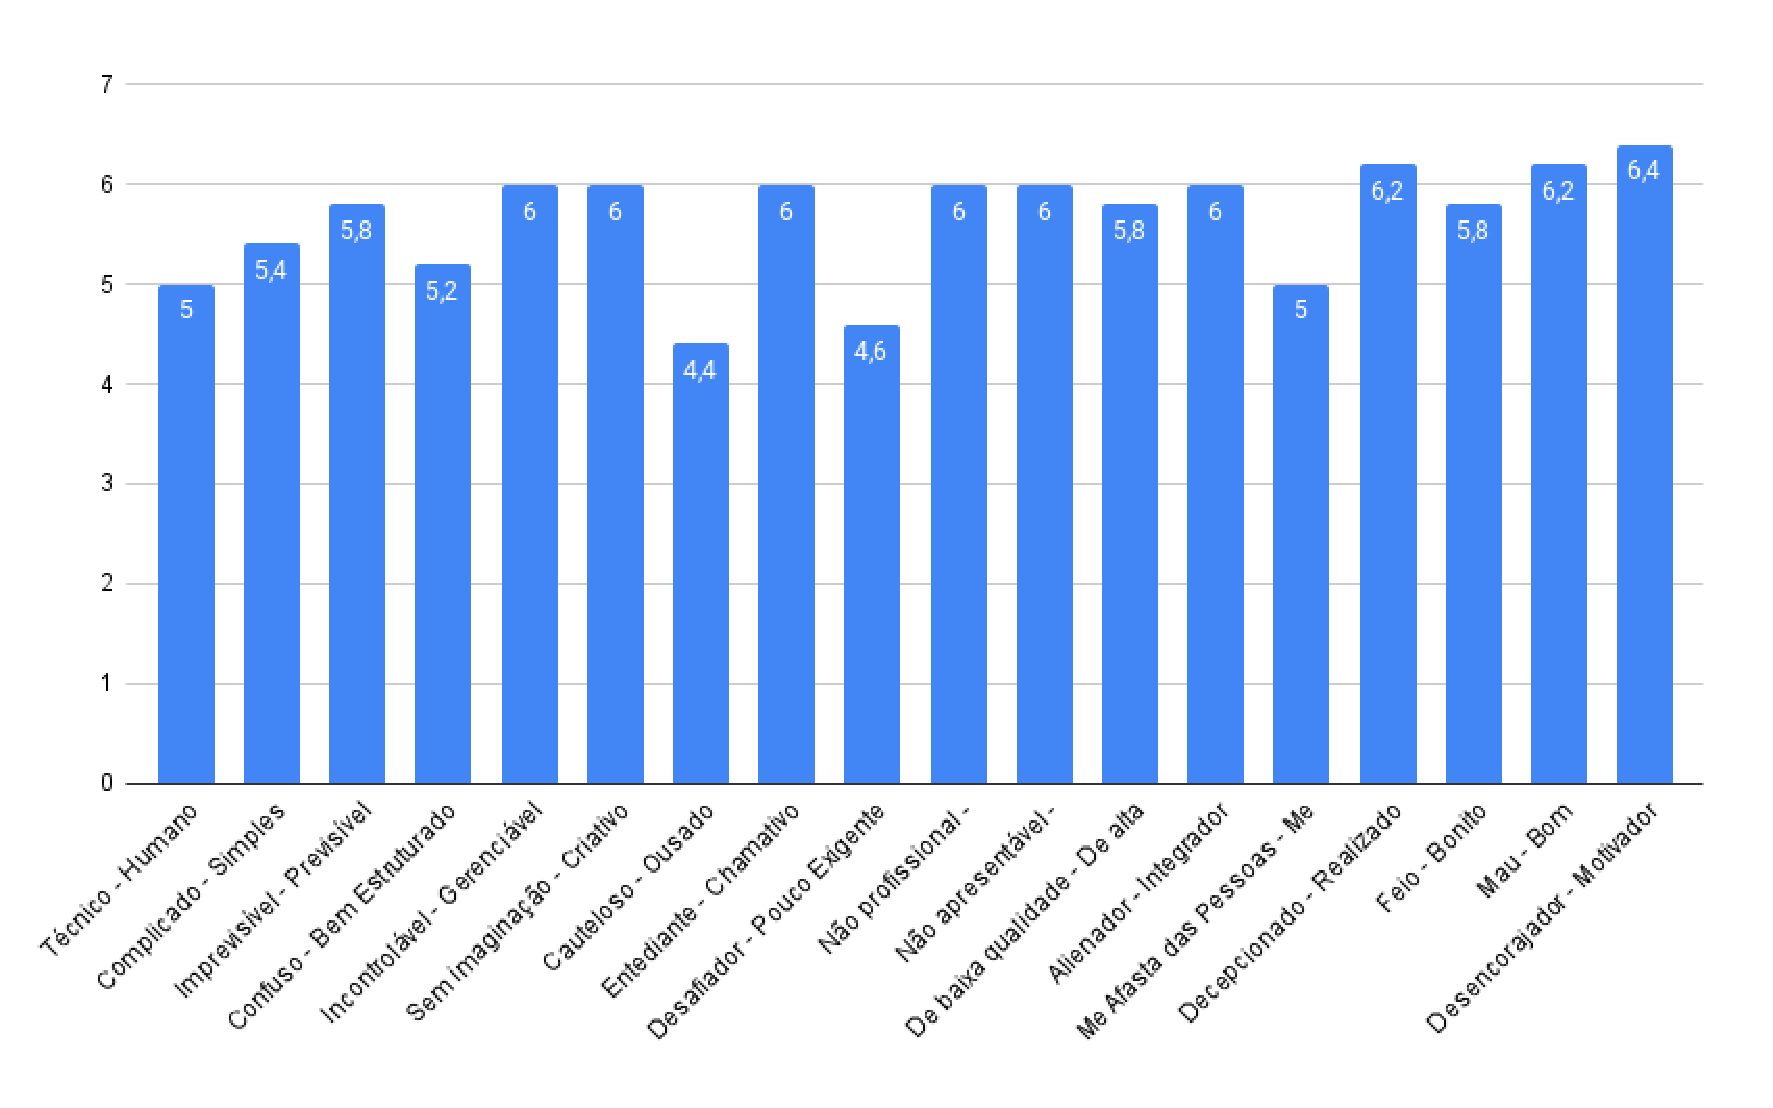
\includegraphics[width=1\textwidth]{figuras/media-geral.eps}
	\end{adjustbox}
	\begin{tablenotes}[flushleft]
		\centering
		\item \textit{Fonte:} Autora.
	\end{tablenotes}
	\label{fig20}
\end{figure}

Já os pares de palavra-chave que revelaram menor satisfação foram: "Cauteloso - Ousado'' e "Confuso - Bem Estruturado''. Isso indica que os participantes perceberam o sistema como mais cauteloso do que ousado, e 
sentiram-se confusos na interação com o sistema. Em suma, e considerando esses \textit{feedbacks}, foi identificado que é necessário focar nas seguintes melhorias: fornecer mais orientações, aprimorar a 
organização e garantir clareza nas informações apresentadas. As Figuras \ref{fig20} e \ref{fig21} ilustram, respectivamente, a média de respostas geral e a média de respostas separadas pelas quatro dimensões principais. 

Ressalta-se que, na média (Figura \ref{fig20}), há aspectos que chamam atenção por seus extremos. "Cauteloso - Ousado'' foi avaliado pelos participantes, obtendo 4,4 como média. Já "Desencorajador - Motivador'' foi avaliado pelos 
participantes com média 6,4. Ao que indica, o aplicativo Multilind pode ser melhorado em "Cauteloso - Ousado''. Já "Desencorajador - Motivador'', em um primeiro momento, não é uma prioridade nas melhorias. Para maior conforto 
quanto à análise dos dados, ressalta-se que valores mais altos, em um intervalo de 0 a 7, representam maior concordância por parte dos participantes no tópico questionado na pergunta, e o inverso é verdadeiro. Na Figura \ref{fig21}, 
reporta-se sobre a maior satisfação dos usuários na dimensão Atratividade, com média na dimensão em 6,15. Em oposição, têm-se as dimensões: Qualidade de Estimulação (Henônica), com média na dimensão em 5,2 (a menor dentre 
as quatro dimensões), e Qualidade Pragmática Percebida, com média na dimensão em 5,48 (segunda menor dentre as quatro dimensões).

\begin{figure}[h!]
	\centering
	\caption{Média \textit{Attrakdiff} por dimensões - Primeiro Ciclo de Testes}
	\begin{adjustbox}{center}
		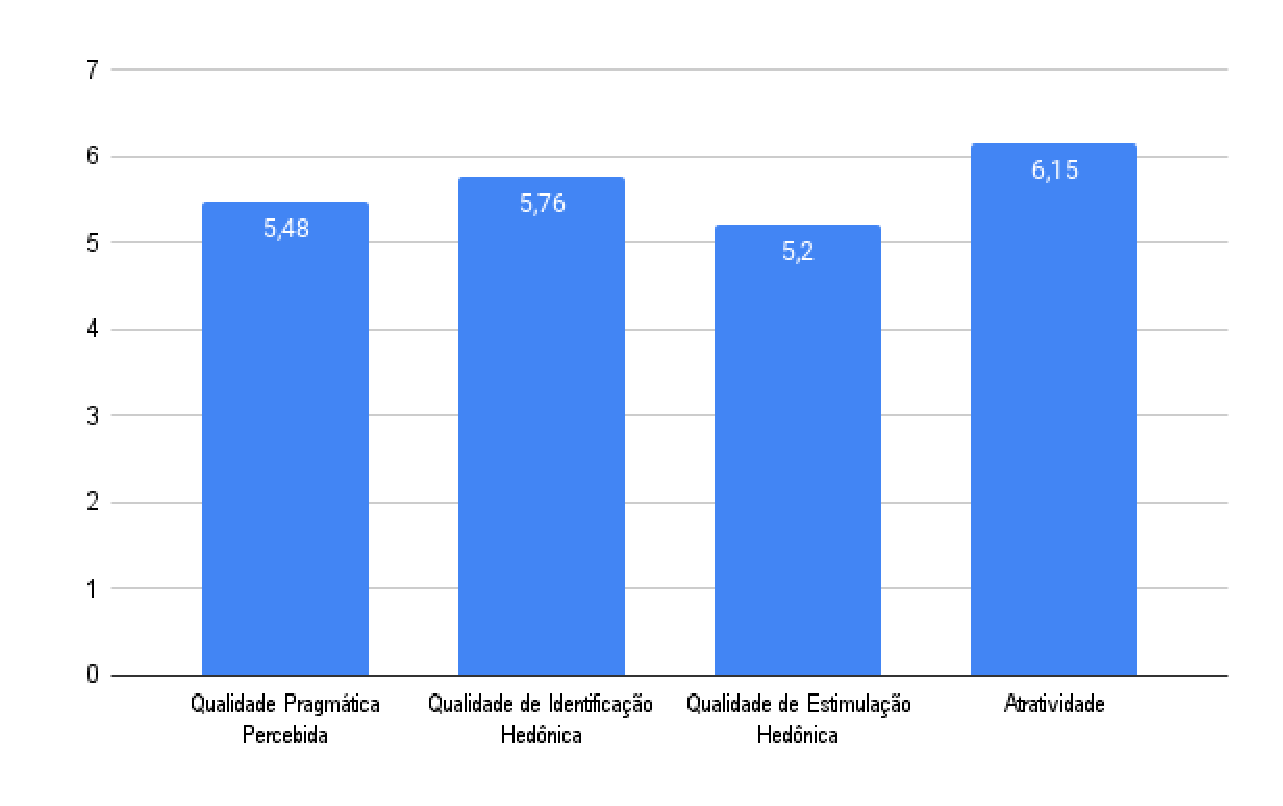
\includegraphics[width=1\textwidth]{figuras/media-separada.eps}
	\end{adjustbox}
	\begin{tablenotes}[flushleft]
		\centering
		\item \textit{Fonte:} Autora.
	\end{tablenotes}
	\label{fig21}
\end{figure}

\section{Segundo Ciclo de Testes}
\label{sec:Segundo Ciclo}
O processo de \textit{design} segue uma abordagem iterativa, ou seja, é uma atividade contínua envolvendo \textit{feedback} constante dos usuários e melhorias incrementais ao longo do tempo. \citeonline{usabilitytest} 
reconhece que nem sempre é possível envolver usuários novos a cada iteração. Portanto, o autor afirma ser possível, com os mesmos usuários, descobrir problemas persistentes e validar melhorias implementadas. 

Após alguns problemas de usabilidade terem sido encontrados no primeiro ciclo de testes, o \textit{design} foi redesenhado\footnote{Protótipo com melhorias. Disponível em: \url{https://shorturl.at/ryEOR}(último acesso: Março 2024)}. 
A segunda rodada de testes com cinco usuários visa mapear os demais problemas de usabilidade que não foram encontrados na primeira rodada de testes, além de aferir se as melhorias realizadas surtiram os efeitos desejados. O segundo estudo poderá aprofundar a 
usabilidade da estrutura fundamental do aplicativo, avaliando questões como arquitetura da informação; fluxo de tarefas, e correspondência com as necessidades do usuário \cite{usabilitytest}.

\subsection{Teste de Usabilidade}
\label{sec:Segundo Teste de Usabilidade}
A Tabela \ref{tab07} apresenta o tempo gasto, considerando cada participante, durante o teste de usabilidade separado por funcionalidade. Considerando os dados, percebem-se melhorias significativas para o caso, por exemplo, da Funcionalidade 04 - Visualizar línguas 
por família linguística, que teve uma redução média de 42,54 segundos. Em seguida, a funcionalidade F01 - Visualizar línguas através do mapa, demonstrou uma redução média de 16,29 segundos. Todas as demais funcionalidades apresentaram considerável redução de 
tempo. 

\begin{table}[h!]
	\centering
	\caption{Tempo gasto por participante - Segundo ciclo de testes}
	\label{tab07}
	\begin{adjustbox}{center}
	\begin{tabular}{l|l|l|l|l|l}
	\hline
	Fucionalidade & Participante 1 & Participante 2 & Participante 3 & Participante 4 & Participante 5 \\ 	\hline
	F01                   & 8.8s     & 12s     & 5,1s      & 9.4s       & 20.1s      \\
	F02                   & 8.4s        & 11.8s      & 8.8s      & 13.9s    & 14.2s     \\
	F03                   & 20.7s        & 4.5s      & 32.9s      & 100s     & 44.4s     \\
	F04                   & 16.1s        & 21.1s     & 89.9s     & 48.1s     & 13.8s     \\
	F05                   & 14.8s      & 18.8s      & 10.8s     & 33s     & 62.7s     \\
	F06                   & 18.4s     & 11.1s      & 14.6s     & 14.4s     & 18.2s     \\
	F07                   & 18.9s     & 20.8s      & 25s     & 21s    & 52.9s       \\ 	\hline
	\end{tabular}
	\end{adjustbox}
	\begin{tablenotes}[flushleft]
		\centering
		\item \textit{Fonte:} Maze. Disponível em: \url{https://app.maze.co/report/Novo-Multilind/hsf4hljyldyqs/intro}.
	  \end{tablenotes}
\end{table}

\subsection{Avaliação da Experiência de Usuário}
\label{sec:Segunda Avaliação da Experiência de Usuário}
No segundo ciclo de avaliação da experiência do usuário, após a conclusão dos testes de usabilidade, os participantes também foram convidados a responder ao Questionário AttrakDiff para analisar a experiência, qualidade e facilidade de uso da aplicação.

A tabela de resultados, presente no Google Sheets, pode ser acessada via o link: 
\url{https://docs.google.com/spreadsheets/d/1H1Rh7tegYa_Ql--i-Xj0oNvzAhHVz_6Xt1jmX3sJEk4/edit?usp=sharing} último acesso: Março 2024, apresenta as avaliações obtidas por meio do Questionário \textit{Attrakdiff} aplicado aos participantes do aplicativo, para o caso 
dessa versão evoluída do protótipo. Além disso, as Figuras \ref{fig28} e \ref{fig29} ilustram a média de respostas geral e a média de respostas separadas pelas quatro dimensões principais, respectivamente.

\newpage

\begin{figure}[h!]
	\centering
	\caption{Média Geral \textit{Attrakdiff} - Segundo Ciclo de Testes}
	\begin{adjustbox}{center}
		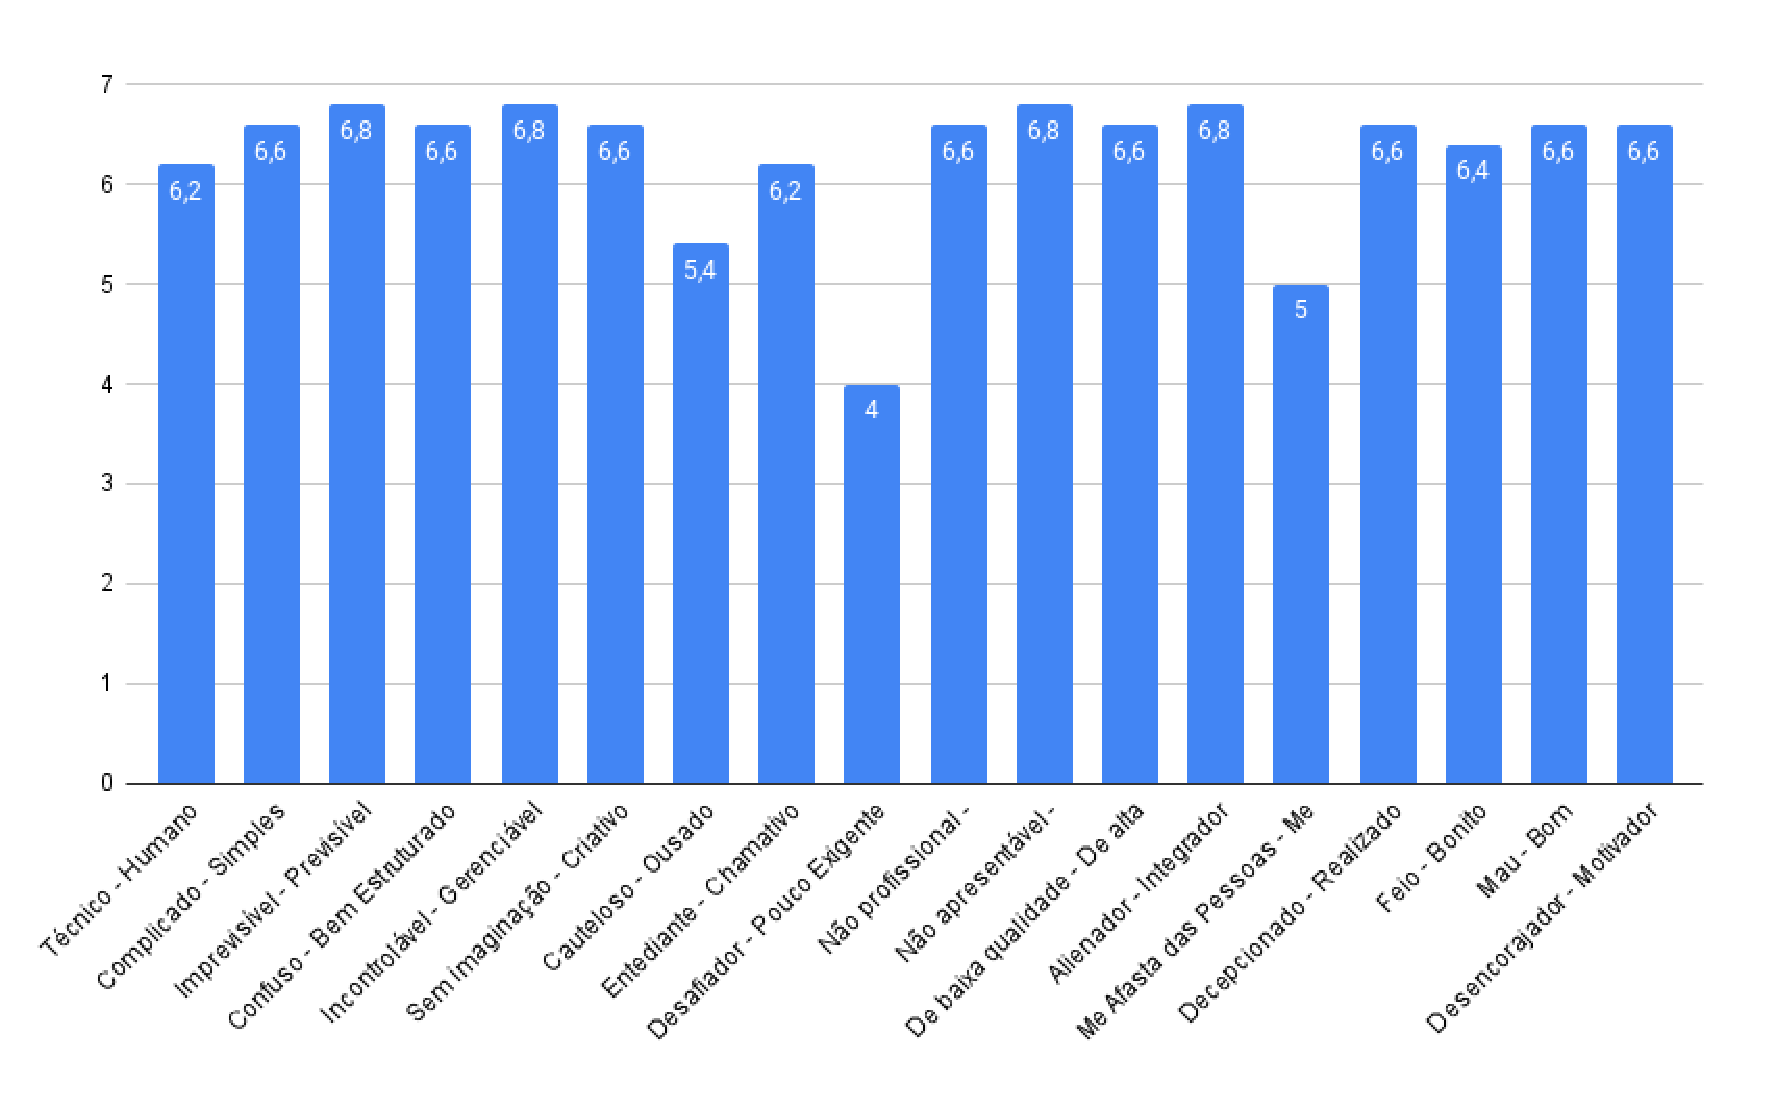
\includegraphics[width=0.8\textwidth]{figuras/media-geral1.eps}
	\end{adjustbox}
	\begin{tablenotes}[flushleft]
		\centering
		\item \textit{Fonte:} Autora.
	\end{tablenotes}
	\label{fig28}
\end{figure}

\begin{figure}[h!]
	\centering
	\caption{Média \textit{Attrakdiff} por dimensões - Segundo Ciclo de Testes}
	\begin{adjustbox}{center}
		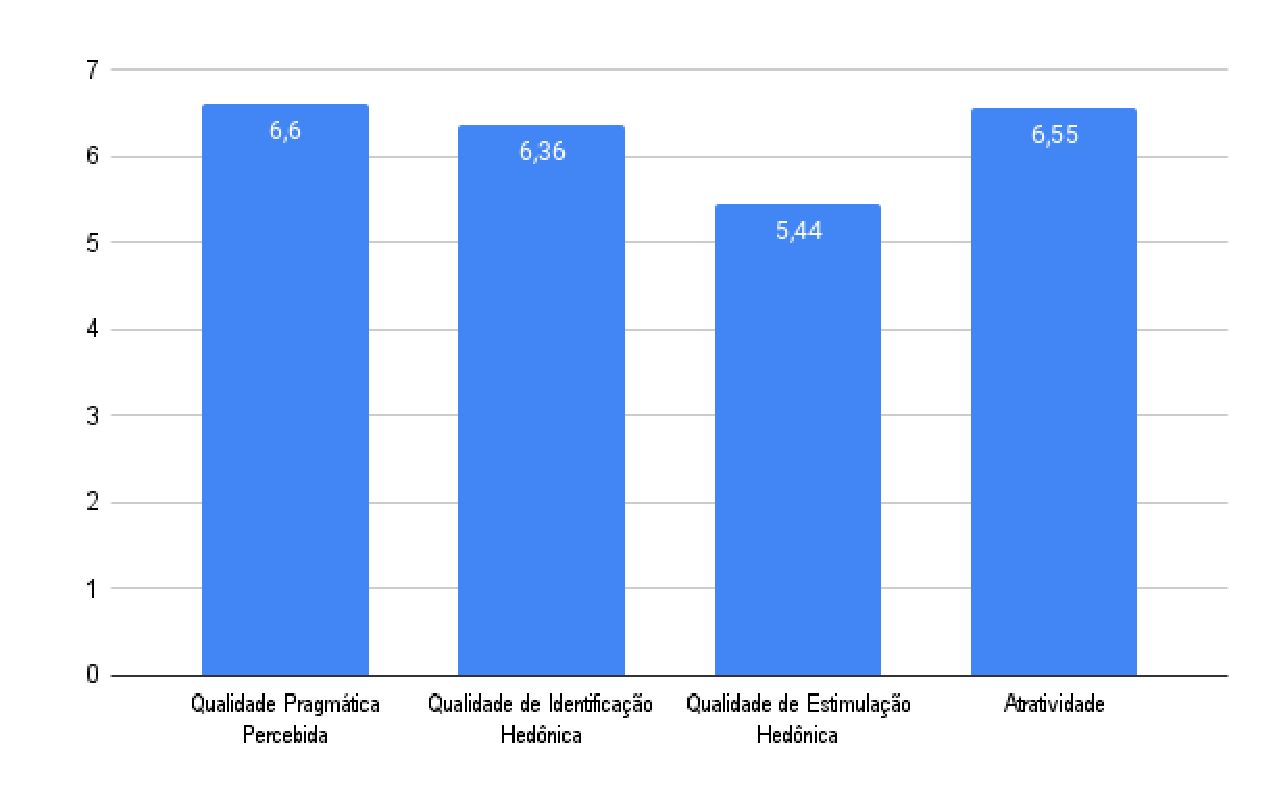
\includegraphics[width=0.8\textwidth]{figuras/media-separada1.eps}
	\end{adjustbox}
	\begin{tablenotes}[flushleft]
		\centering
		\item \textit{Fonte:} Autora.
	\end{tablenotes}
	\label{fig29}
\end{figure}

Com base nos resultados do segundo ciclo de testes, foi elaborado um gráfico para apresentar uma visão geral da pontuação alcançada em cada par de palavras avaliadas pelo Questionário AttrakDiff. Analisando os dados obtidos, observa-se que alguns pares de palavras-chave 
se destacaram positivamente. Por exemplo, "Imprevisível - Previsível" e "Incontrolável - Gerenciável" receberam pontuações altas, indicando uma boa percepção dos usuários em relação à previsibilidade e ao controle oferecidos pela aplicação.

No entanto, houve alguns pares de palavras que revelaram menor satisfação por parte dos participantes, como "Confuso - Bem Estruturado" e "Cauteloso - Ousado". Esses resultados sugerem a necessidade de fornecer mais orientações e aprimorar a organização da aplicação 
para garantir uma experiência mais clara e intuitiva para os usuários.

Ao analisar a média das respostas por dimensão, destaca-se que a qualidade pragmática percebida obteve uma pontuação significativa de 6.6, indicando uma percepção positiva dos usuários em relação à eficiência e facilidade de uso da aplicação para atender às suas necessidades 
e objetivos. A qualidade de identificação hedônica também apresentou uma melhoria considerável, alcançando uma média de 6.36. Já a qualidade de estimulação hedônica teve uma leve melhoria, atingindo uma média de 5.44. Por fim, a atratividade geral da aplicação registrou um aumento, 
alcançando uma média de 6.55, o que indica uma melhoria na percepção dos usuários sobre a qualidade visual e o apelo geral da aplicação.

Mesmo diante dos resultados positivos, novas possíveis melhorias também foram pontuadas durante o segundo ciclo de testes, com destaque para:

\begin{itemize}
	\item Português Indígena: Alguns usuários expressaram preocupação em relação à tradução para o português indígena, visto que não se trata de uma língua única, mas sim uma variação do português brasileiro que depende de alguns fatores, como contato linguístico com outros 
	povos, região do Brasil, identidade cultural e grau de preservação da língua nativa;
	\item Participação Coletiva: Com objetivo de maior participação de falantes das línguas, a opção de reportar em caso de erro de tradução ou inconsistência foi sugerida. Tal funcionalidade visa aumentar a confiabilidade dos dados presentes no aplicativo, além de incentivar a 
	participação dos povos indígenas na documentação das línguas, e
	\item Pronúncia de Palavras: A língua oral é a principal forma de comunicação e expressão cultural para muitos povos indígenas. Por isso, introduzir uma funcionalidade de pronúncia pode ser uma ótima maneira de ajudar os usuários a compreender palavras de maneira mais clara 
	e precisa.
\end{itemize}

\section{Impressão dos Resultados}
\label{sec:Impressão dos Resultados}
Nesta seção, uma análise detalhada dos resultados obtidos nos ciclos de testes conduzidos para avaliar a usabilidade e a experiência do usuário é conferida. Os dados coletados foram examinados, levando em consideração os \textit{feedbacks} dos participantes, as métricas de 
tempo para realizar tarefas, o sucesso direto ou indireto de tarefas na interação com o aplicativo, a quantidade de cliques errados e as médias do \textit{AttrakDiff}.

\subsection{Percepção Geral dos Usuários}
\label{sec:Percepção Geral dos Usuários}
No primeiro ciclo de testes, conduzido com um grupo inicial de usuários, foram identificados diversos pontos que necessitavam de aperfeiçoamento para melhorar a usabilidade e experiência de usuário. Entre os principais \textit{feedbacks} estavam a falta de orientação no primeiro uso, 
dificuldades na localização de funcionalidades, ausência de cores vibrantes e falta de informações sobre como contribuir com a base de dados do aplicativo.

No segundo ciclo de testes, conduzido com o mesmo grupo de usuários após as melhorias implementadas, os participantes relataram uma melhor compreensão da aplicação devido ao passo a passo inicial e à validação das mudanças nos fluxos do aplicativo. Especificamente, a visualização da 
família linguística, a mudança no dicionário para exibir as palavras na língua indígena e a disposição das imagens de uma palavra específica, contribuindo para uma experiência mais satisfatória no uso do aplicativo.

\subsection{Análise de Usabilidade}
\label{sec:Análise de Usabilidade}

\subsubsection{Primeiro Ciclo de Testes}
\label{sec:Primeiro Ciclo de Testes}

No primeiro ciclo de testes, houve uma grande variação nas taxas de sucesso direto, com algumas tarefas atingindo 100\% de sucesso, enquanto outras apresentaram uma taxa de 0\%. Essa disparidade evidencia uma inconsistência na usabilidade das diferentes funcionalidades do aplicativo.

Entre as tarefas avaliadas, a F01 se destacou com uma taxa de sucesso direto de 100\%. Esta tarefa envolve a visualização de línguas através do mapa e não foi alterada entre os ciclos de testes devido ao seu alto sucesso direto. Isso sugere que os participantes conseguiram realizar essa 
tarefa sem encontrar dificuldades significativas, contribuindo para a usabilidade da aplicação.

Por outro lado, as taxas de cliques errados durante o primeiro ciclo de testes foram motivo de preocupação, variando entre 15.2\% e 69.8\%. Esses resultados apontam para uma execução menos eficaz das tarefas, indicando possíveis problemas de usabilidade ou falta de clareza nas instruções 
fornecidas aos usuários.

Em relação à duração média para concluir as tarefas, destaca-se a tarefa F04 - Visualizar línguas por família linguística, apresentando uma duração média bastante elevada de 198.4 segundos (ou aproximadamente 3.3 minutos). Isso sugere dificuldades substanciais na execução 
dessa tarefa por parte dos participantes. Da mesma forma, a tarefa F07 - Visualizar imagens relativas às palavras de uma língua, teve uma duração média de 65.3 segundos.

Além disso, é importante notar que ambas as tarefas, F04 e F07, apresentaram uma taxa de sucesso direto de 0\%. Esses resultados indicam não apenas a complexidade das tarefas, mas também dificuldades significativas por parte dos participantes em concluí-las sem cometer erros. 

\subsubsection{Segundo Ciclo de Testes}
\label{sec:Segundo Ciclo de Testes}
No segundo ciclo de testes, foi possível notar melhorias nas métricas de usabilidade coletadas pelo Maze. As taxas de sucesso direto foram mais consistentes, com todas as tarefas apresentando taxas de sucesso direto acima de 20\%, indicando uma melhoria na usabilidade das 
funcionalidades do aplicativo. Adicionalmente, as taxas de cliques errados foram, em geral, mais baixas em comparação com o primeiro ciclo, sugerindo uma melhoria na clareza das funções disponíveis na aplicação.

Em relação à duração média para concluir as tarefas, o segundo ciclo de testes apresentou melhorias significativas, especialmente nas tarefas F04 e F07. No primeiro ciclo de testes, a tarefa F04 - Visualizar línguas por família linguística, que apresentava duração média de 
198.4 segundos, teve uma redução para 37.8 segundos no segundo ciclo. Além do mais, a taxa de sucesso direto aumentou de 0\% no primeiro ciclo para 60\% no segundo ciclo.

Quanto à tarefa F07 - Visualizar imagens relativas às palavras de uma língua, que tinha uma duração média de 65.3 segundos, foi reduzida para 27.7 segundos. Além disso, a taxa de sucesso direto aumentou de 0\% no primeiro ciclo para 40\% no segundo, evidenciando uma evolução 
significativa na capacidade dos usuários em completar a tarefa com sucesso. A taxa de cliques errados, ainda, diminuiu de 54.3\% para 27.7\%, demonstrando uma interação mais precisa no segundo \textit{design}.

\subsection{Análise da Experiência de Usuário}
\label{sec:Análise da Experiência de Usuário}

\subsubsection{Primeiro Ciclo de Testes}
\label{sec:Primeiro Ciclo de Testes2}
Durante o primeiro ciclo de testes, os participantes avaliaram a aplicação através do Questionário \textit{AttrakDiff}. Os resultados revelaram que o par "Cauteloso - Ousado" obteve a menor média de 4,4, indicando uma percepção mais cautelosa do sistema por parte dos usuários. O par 
"Desafiador - Pouco Exigente" teve a segunda menor média, sinalizando que os usuários acharam a aplicação desafiadora de ser utilizada.

Por outro lado, o par "Desencorajador - Motivador" recebeu a maior média de 6,4, sugerindo uma percepção mais positiva em relação à motivação proporcionada pela aplicação. Na dimensão Atratividade, a média foi de 6,15, demonstrando uma boa percepção visual da aplicação. Entretanto, 
na Qualidade de Estimulação (Hedônica), a média foi de 5,2, indicando uma percepção moderada em relação à capacidade da aplicação de estimular os usuários. Similarmente, na dimensão Qualidade Pragmática Percebida, a média foi de 5,48, sugerindo uma percepção moderada em relação à 
eficácia percebida da aplicação em atender às necessidades dos usuários.

\subsubsection{Segundo Ciclo de Testes}
\label{sec:Segundo Ciclo de Testes2}
No segundo ciclo de testes, os usuários destacaram uma maior clareza na compreensão da aplicação devido ao passo a passo inicial e à validação das mudanças nos fluxos do aplicativo, que se mostraram mais intuitivos. Os dados revelam melhorias em todas as quatro dimensões principais do 
\textit{AttrakDiff}, que avalia a experiência do usuário. 

A Qualidade Pragmática Percebida, que mede o grau de sucesso e esforço que os usuários têm ao utilizar o aplicativo para atingir seus objetivos, teve uma melhora significativa, anteriormente de 5,48 para 6,6. Em relação à 
Qualidade Hedônica-Identidade, pode-se notar uma melhoria considerável, atingindo 6,36. Essa dimensão representa o grau de identificação da aplicação com o usuário. Já a Qualidade Hedônica-Estímulo, indica a quantidade de apoio que a aplicação oferece ao usuário 
para desenvolver, estimular e aumentar a motivação. Uma pequena melhora pode ser notada, de 5,2 para 5,44. Por fim, é importante destacar que a atratividade da aplicação, que representa uma classificação geral, apresentou uma melhora de 0,4 pontos, alcançando a 
pontuação de 6,55.

\subsection{Considerações Finais}
\label{sec:Considerações Finais}
Neste capítulo, os resultados dos testes de usabilidade e experiência do usuário no aplicativo Multilind são apresentados. O capítulo começa discutindo as \hyperref[sec:Personas]{Personas} envolvidas nos testes, seguido pelos \hyperref[sec:Cenários de Uso]{Cenários de Uso} que foram avaliados. 
As \hyperref[sec:Práticas Adotadas]{Práticas Adotadas} durante os testes, incluindo o uso da ferramenta Maze para registro de métricas, são descritas em detalhes.

No geral, os resultados dos testes sugerem que as melhorias implementadas tiveram um impacto positivo na usabilidade e experiência do usuário no aplicativo Multilind. O aumento mais significativo em relação às estatísticas foi na Qualidade Pragmática Percebida. Esta refere-se à percepção 
do usuário em relação às funcionalidade, eficiência e facilidade de uso. Portanto, indica a facilidade dos usuários em atender suas necessidades e seus objetivos.